\documentclass[12pt,preprint]{aastex}
\usepackage{geometry,amsmath}
\usepackage{float}
%\usepackage{titlesec} %used to format titles
\usepackage{graphicx} %for handling figures
\usepackage[none]{hyphenat} %disallows hyphenated words


\begin{document}

\title{HERA Dish Reflectometry} 
\author{Zaki Ali, Carina Cheng, Aaron Parsons, Nipanjana Patra}
\maketitle

\section{Introduction}

*motivation for these measurements*

*explain the spec of -60dB at 60ns*

\section{Set-Up}

A prototype 14-m HERA dish has been built at the NRAO site in Green Bank, West Virginia. It is a parabolic dish supported by 10 wood poles with PVC piping along the rim and towards the central hub. Wire mesh covers the dish. A PAPER feed enclosed in a metal cylindrical cage is suspended over the center of the dish (to prevent feed-to-feed interaction between neighboring dishes) and connected to three pulleys which are able to lower and raise the feed. 

\begin{figure}[H]
\centering
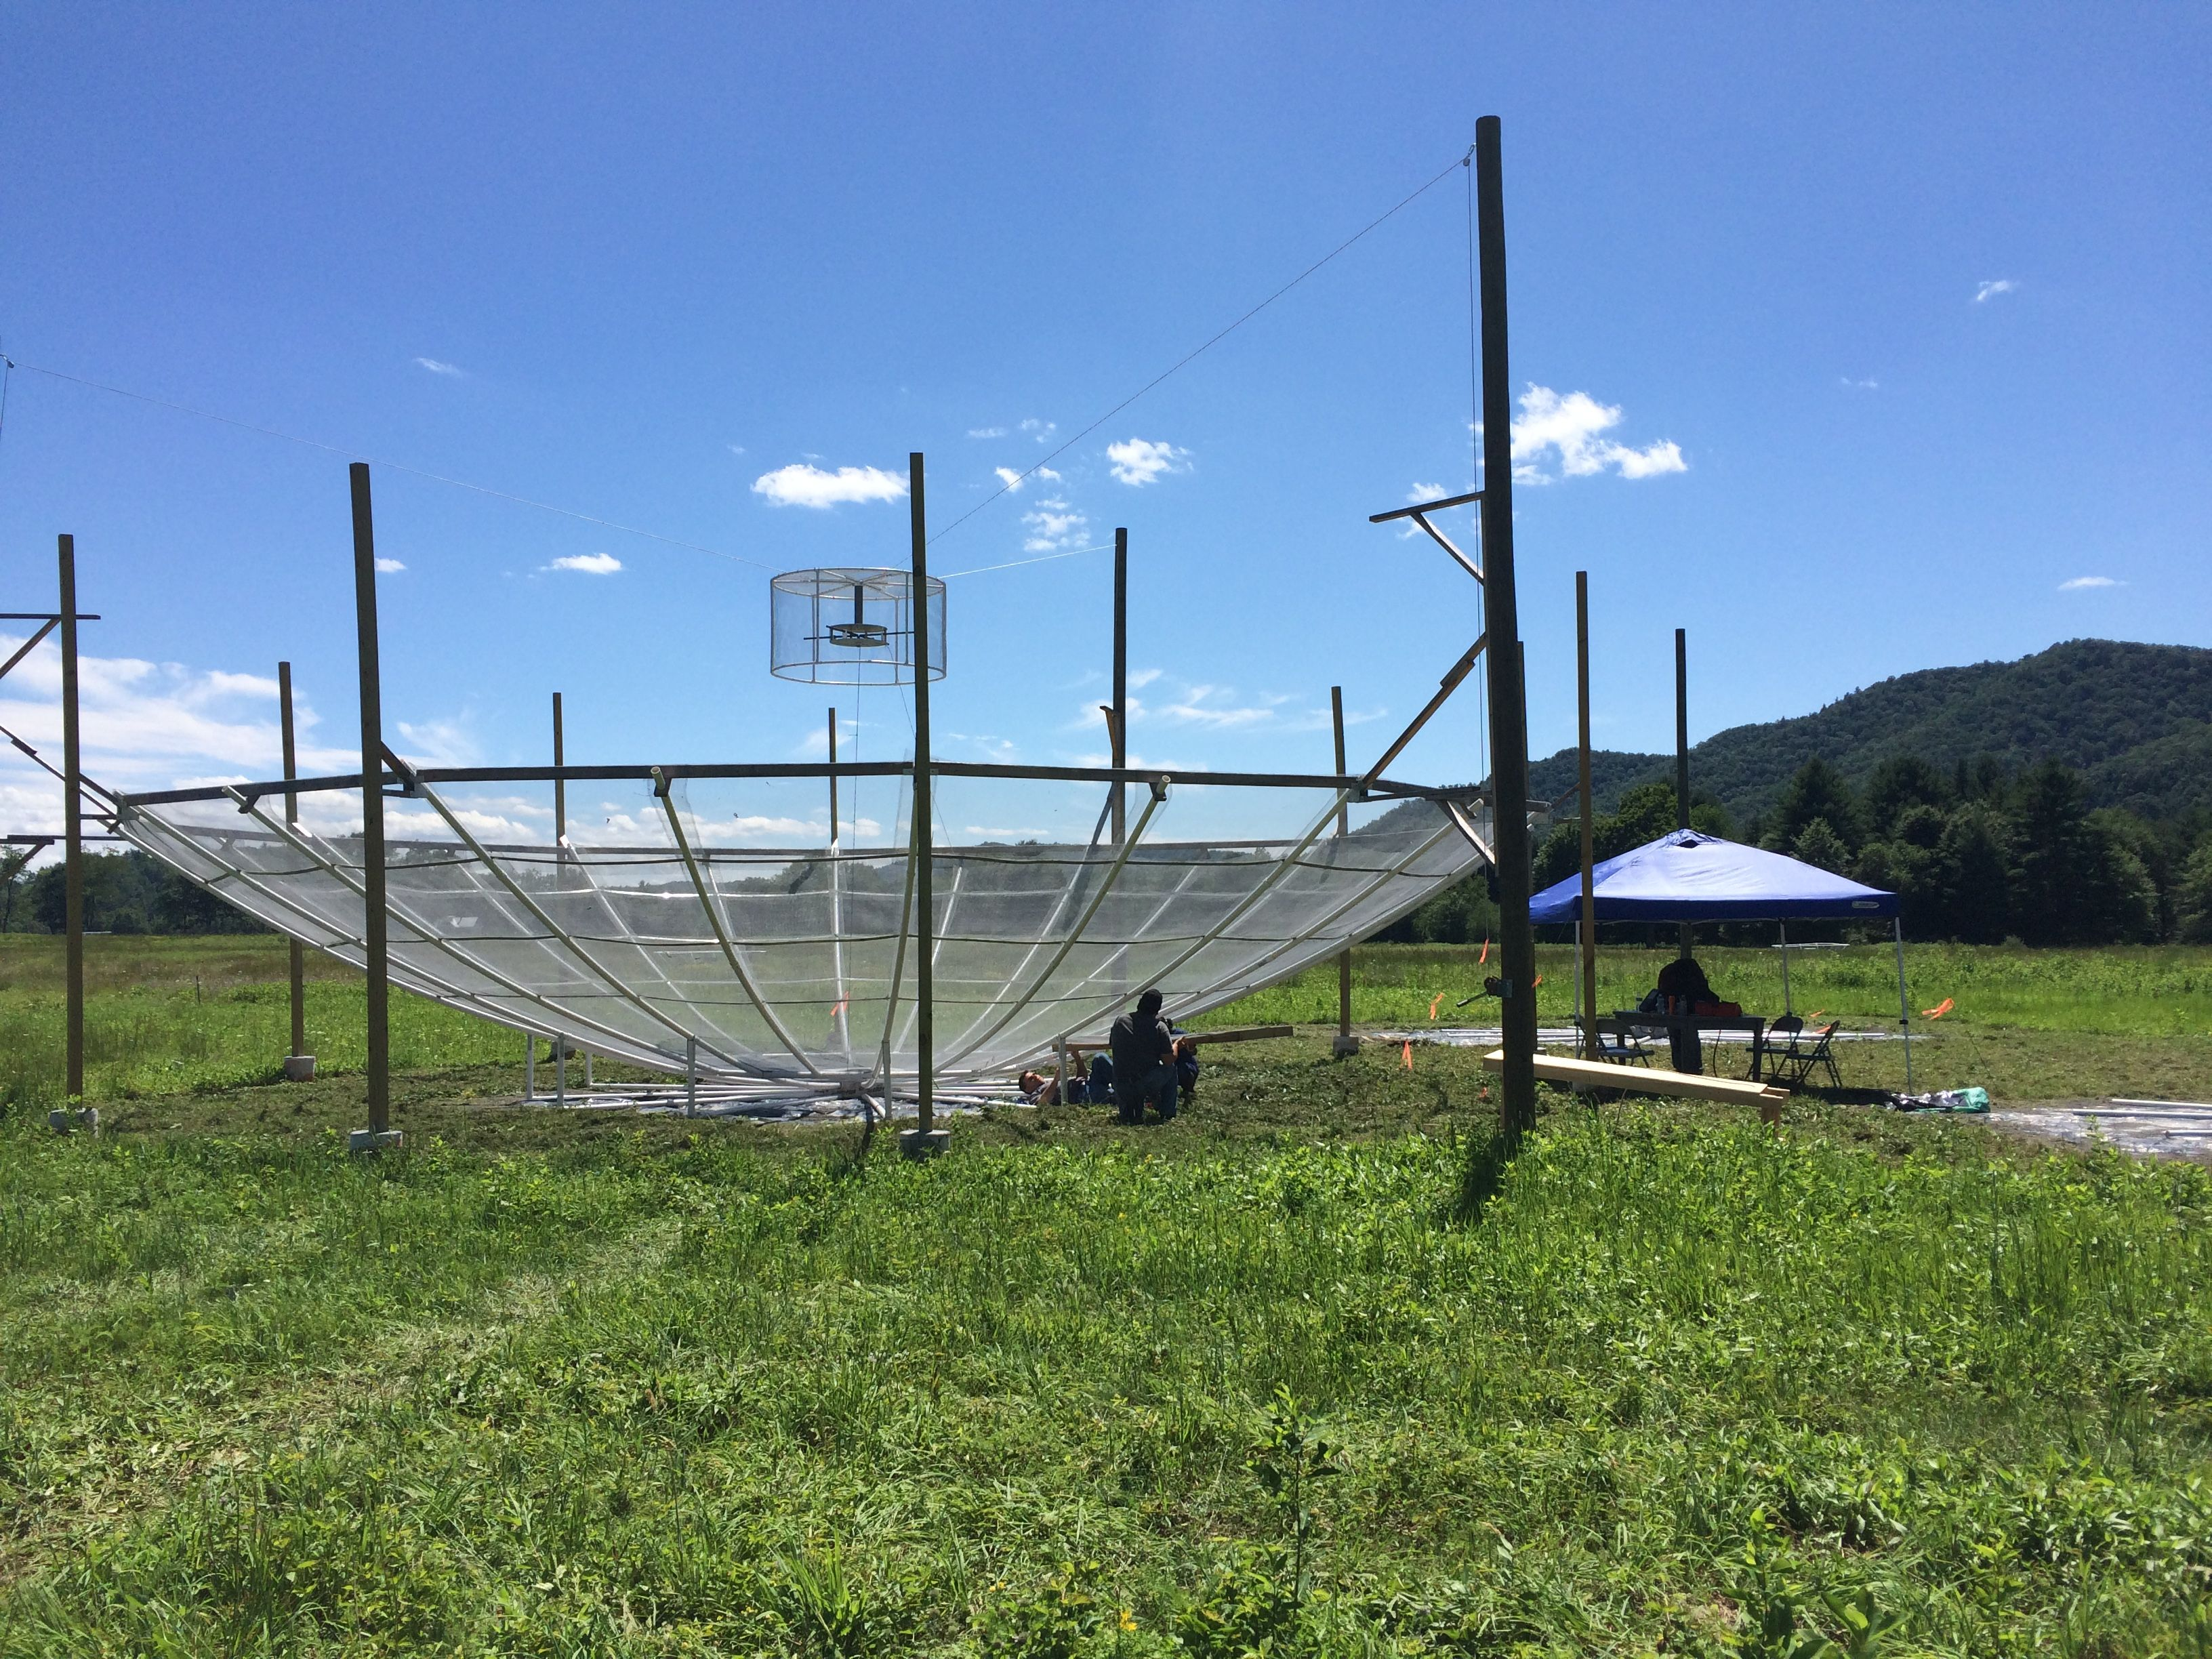
\includegraphics[trim={2cm 20cm 30cm 15cm},clip, totalheight=0.45\textheight]{plots/heradish.jpg}
\caption{HERA dish and feed at the Green Bank NRAO site.}
\end{figure}

We took reflectometry measurements on July 20-23, 2015 using a FieldFox Network Analyzer. A pulse was generated and sent through a 75ft long cable (50$\Omega$ impedance) that connected to the feed with a 4:1 active balun. This signal gets transmitted through the feed and then reflects off the dish...

\section{Theory}

*compare cable pulse measurements vs. actual sky measurements and how the amount of signal that is transmitted/reflected is different*

*explain why the level of the measurements has to be brought down, and how this is okay for high delays*

\begin{figure}[H]
\centering
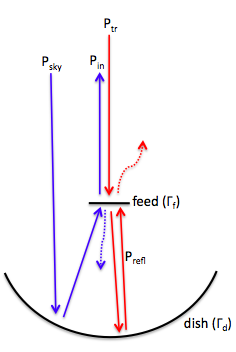
\includegraphics[totalheight=0.5\textheight]{plots/reflection_cartoon.png}
\caption{The blue solid lines represent an original sky signal entering the feed. A small percentage of it (dashed blue) is reflected off the dish, and it is these reflections that we are concerned about. In our measurements however, the reflections measured contain most of the original pulse signal (solid red), so it is crucial to adjust for this difference in our analysis.}
\end{figure}


\section{Measurements}

We begin with a reflectometry measurement with the feed suspended at 12 ft (distance between the balun and top of the central hub) for a frequency bandwidth of 50MHz - 500MHz.

\begin{figure}[H]
\centering
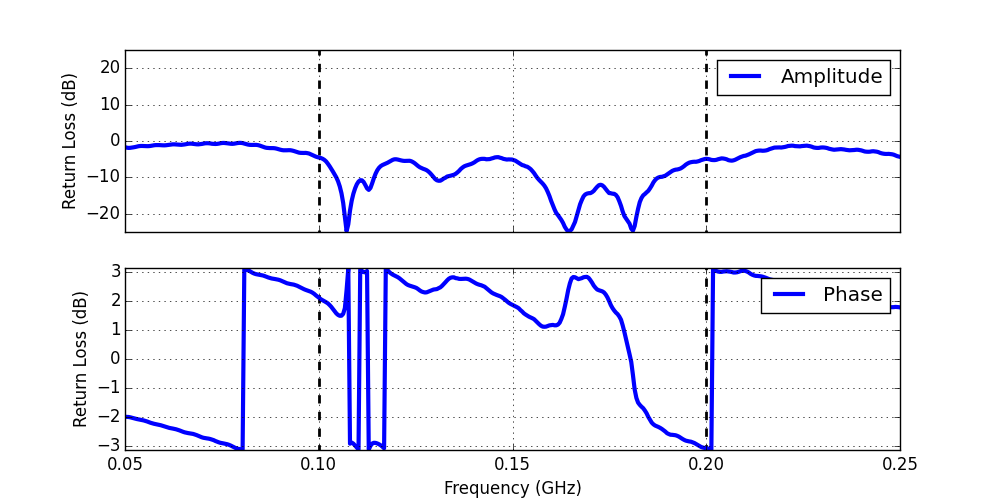
\includegraphics[totalheight=0.4\textheight]{plots/frequency_amp_phase.png}
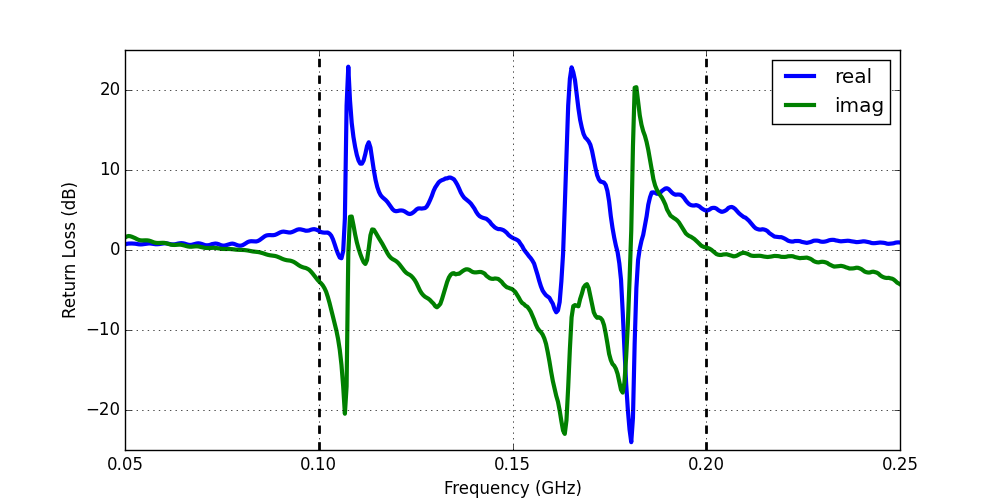
\includegraphics[totalheight=0.4\textheight]{plots/frequency_real_imag.png}
\caption{Top: Amplitude and phase of the reflected signal. Bottom: Real part and imaginary part of the reflected signal.}
\end{figure}

Next, we Fourier-transform along the frequency axis for 3 selected bandwidths: 50MHz-250MHz (the HERA bandwidth), 100MHz-200MHz (the PAPER bandwidth), and 140MHz-160MHz (bandwidth particularly relevant for making power spectra). This produces delay plots that shows...

\begin{figure}[H]
\centering
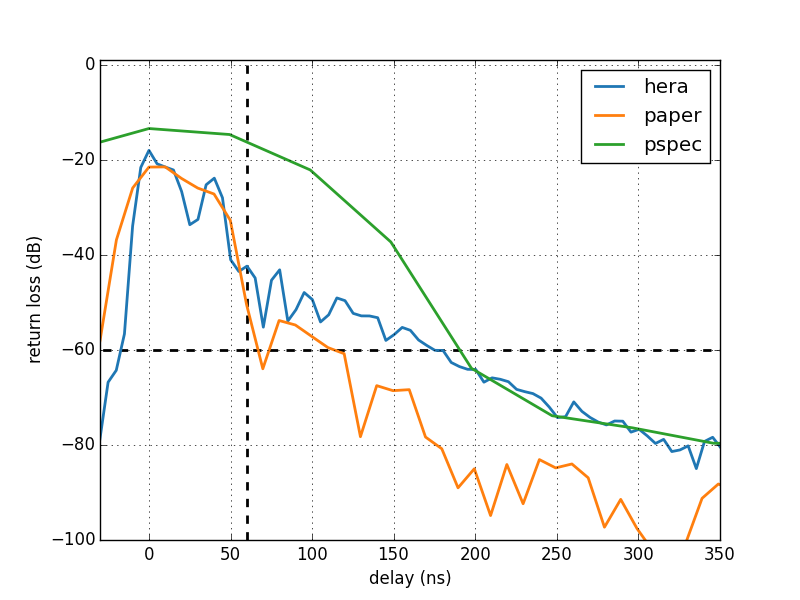
\includegraphics[totalheight=0.5\textheight]{plots/delay3_window.png}
\caption{Delay plots produced using a Blackman-Harris window function for 3 different frequency bandwidths.}
\end{figure}

The importance of window functioning when Fourier-transforming is illustrated in Figure...

\begin{figure}[H]
\centering
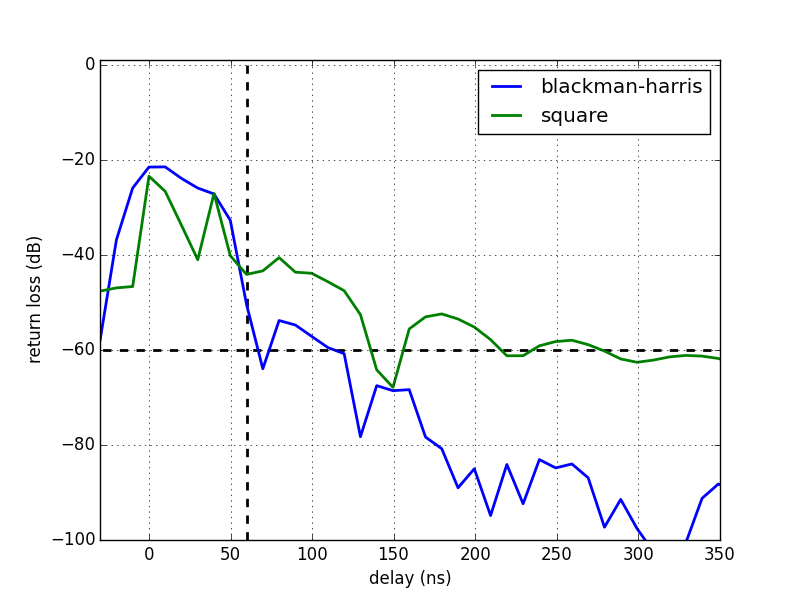
\includegraphics[totalheight=0.5\textheight]{plots/bh_vs_sq.png}
\caption{Delay plot produced using a Blackman-Harris window function vs. a square window function for the PAPER bandwidth.}
\end{figure}

Finally, more robust measurements are taken with the feed at varying heights (6ft, 9ft, 12ft, and 15ft)...

\begin{figure}[H]
\centering
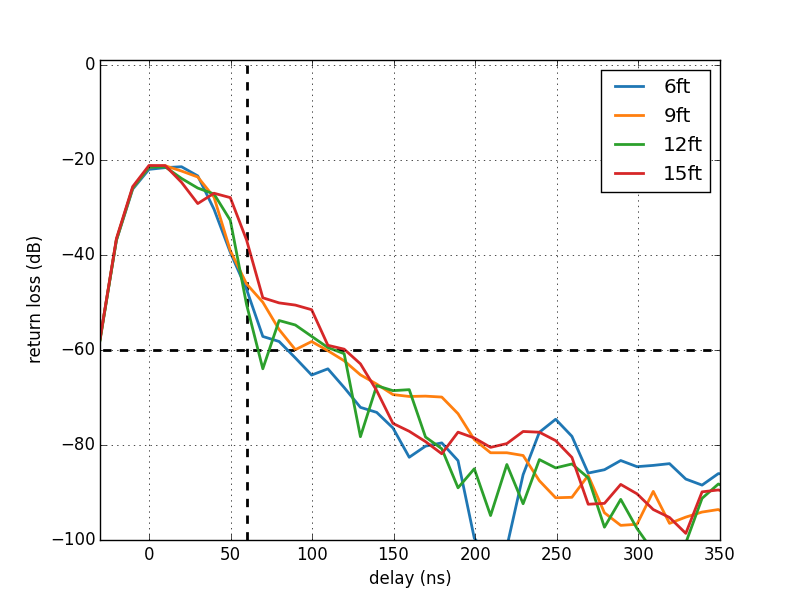
\includegraphics[totalheight=0.5\textheight]{plots/delay_heights_paper.png}
\caption{Delay plots produced using a Blackman-Harris window function for 4 different feed heights and the PAPER bandwidth.}
\end{figure}

\begin{figure}[H]
\centering
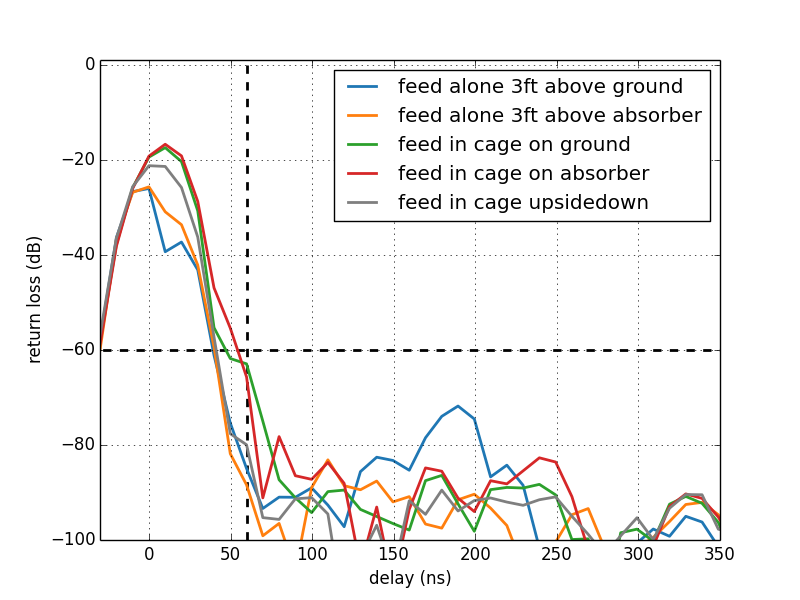
\includegraphics[totalheight=0.5\textheight]{plots/delay_feed.png}
\caption{Delay plots produced using a Blackman-Harris window function for different lone feed configurations and the PAPER bandwidth.}
\end{figure}


\section{Discussion}

\section{Conclusion}


\end{document}
